\section{Segunda Versi\'on de Round Robin}

La segunda versi\'on de round robin impide el pasaje de una tarea de un core a otro, de acuerdo a lo que requiere el \textbf{ejercicio 8}. De manera que en la carga del proceso se determina a qu\'e core tiene que estar asignado. El criterio para tomar esta decisi\'on se basa en la cantidad de tareas asociadas a un core: la nueva tarea que entra al sistema ir\'a a aquel core que tenga asignadas menos tareas en estado RUNNING o BLOCKED o READY.
Esta segunda versi\'on de \textit{round robin} se encuentra implementada en los archivos \verb+sched_rr2.h+ y \verb+sched_rr2.cpp+.

Para implementarla se us\'o un vector de colas. En el header \verb+sched_rr2.h+ se define este vector como un atributo privado.

Por otra parte, tenemos otro atributo privado, que guarda las tareas asignadas a cada core:

\begin{verbatim}
        std::vector< std::queue<int> > qs; // guarda las colas de prioridades asignadas 
                                           //a cada nucleo
        std::vector< std::vector<int> > nucleos; // guarda las tareas 
                                                 // asignadas a cada nucleo
\end{verbatim}

En el constructor del SchedRR2, inicializamos los vectores. Creamos tantas colas y vectores como cores existan en el ambiente:

\begin{verbatim}
SchedRR2::SchedRR2(vector<int> argn) {
	// Round robin recibe la cantidad de cores y sus cpu_quantum por parámetro
    unsigned int cantidadCores = argn[0];
    for (unsigned int i = 0; i < cantidadCores; i++) {
        queue<int> pids;
        vector<int> procesos;
        qs.push_back(pids);
        nucleos.push_back(procesos);
    }
}

\end{verbatim}

Cuando una tarea entra al sistema, se carga y se la asignamos al core que tiene menos tareas a\'no terminadas asociadas. Para ello iteramos por cada de las colas para ver cu\'al tiene menor cantidad:

\begin{verbatim}
    unsigned int nucleoMenosCongestionado = 0;
    unsigned int cantidadEnNucleoMenosCongestionado = qs[0].size();
    for (unsigned int i = 0; i < qs.size(); i++) { // se iteran todos los nucleos para ver
                        // cual es el menos congestionado
        if (qs[i].size() < cantidadEnNucleoMenosCongestionado) {
            nucleoMenosCongestionado = i;
            cantidadEnNucleoMenosCongestionado = qs[i].size();
        }
      }

     qs[nucleoMenosCongestionado].push(pid); // se pushea a este nucleo
      nucleos[nucleoMenosCongestionado].push_back(pid); // se lo asocia al nucleo                         
      //menos congestionado

\end{verbatim}

La selecci\'on para la siguiente tarea a ejecutarse, es similar a SchedRR, con la diferencia de que se consideran solamente la cola asociada al core que envi\'o la interrupci\'on de reloj. Lo mismo ocurre en el caso del desbloqueo. La tarea se vuelve a asociar a la cola a la que se vincul\'o en el momento de la carga.

La otra diferencia a tener en cuenta es que cuando una tarea termina, no solamente se desencola sino que se elimina del vector que tiene las tareas asociadas al core en donde culmin\'o su ciclo de vida.

El primer experimento que hicimos consiste en ejecutar el siguiente lote de tareas:

\begin{verbatim}
TaskCPU 3
TaskCPU 3
TaskCPU 3
TaskCPU 3
TaskCPU 3
\end{verbatim}

con 2 cores, tomando como overhead de cambio de core 1, 2, 3 y 4 quantums. El tiempo de cambio de contexto se mantuvo en 1 en cada una de las mediciones. Se hizo este experimento para verificar c\'omo incid\'ia el cambio del overhead de cambio de core. 


\begin{figure}[H]
\caption{SchedRR 5 TaskCPU 2 cores 1, 2, 3, 4 para cambio de core}
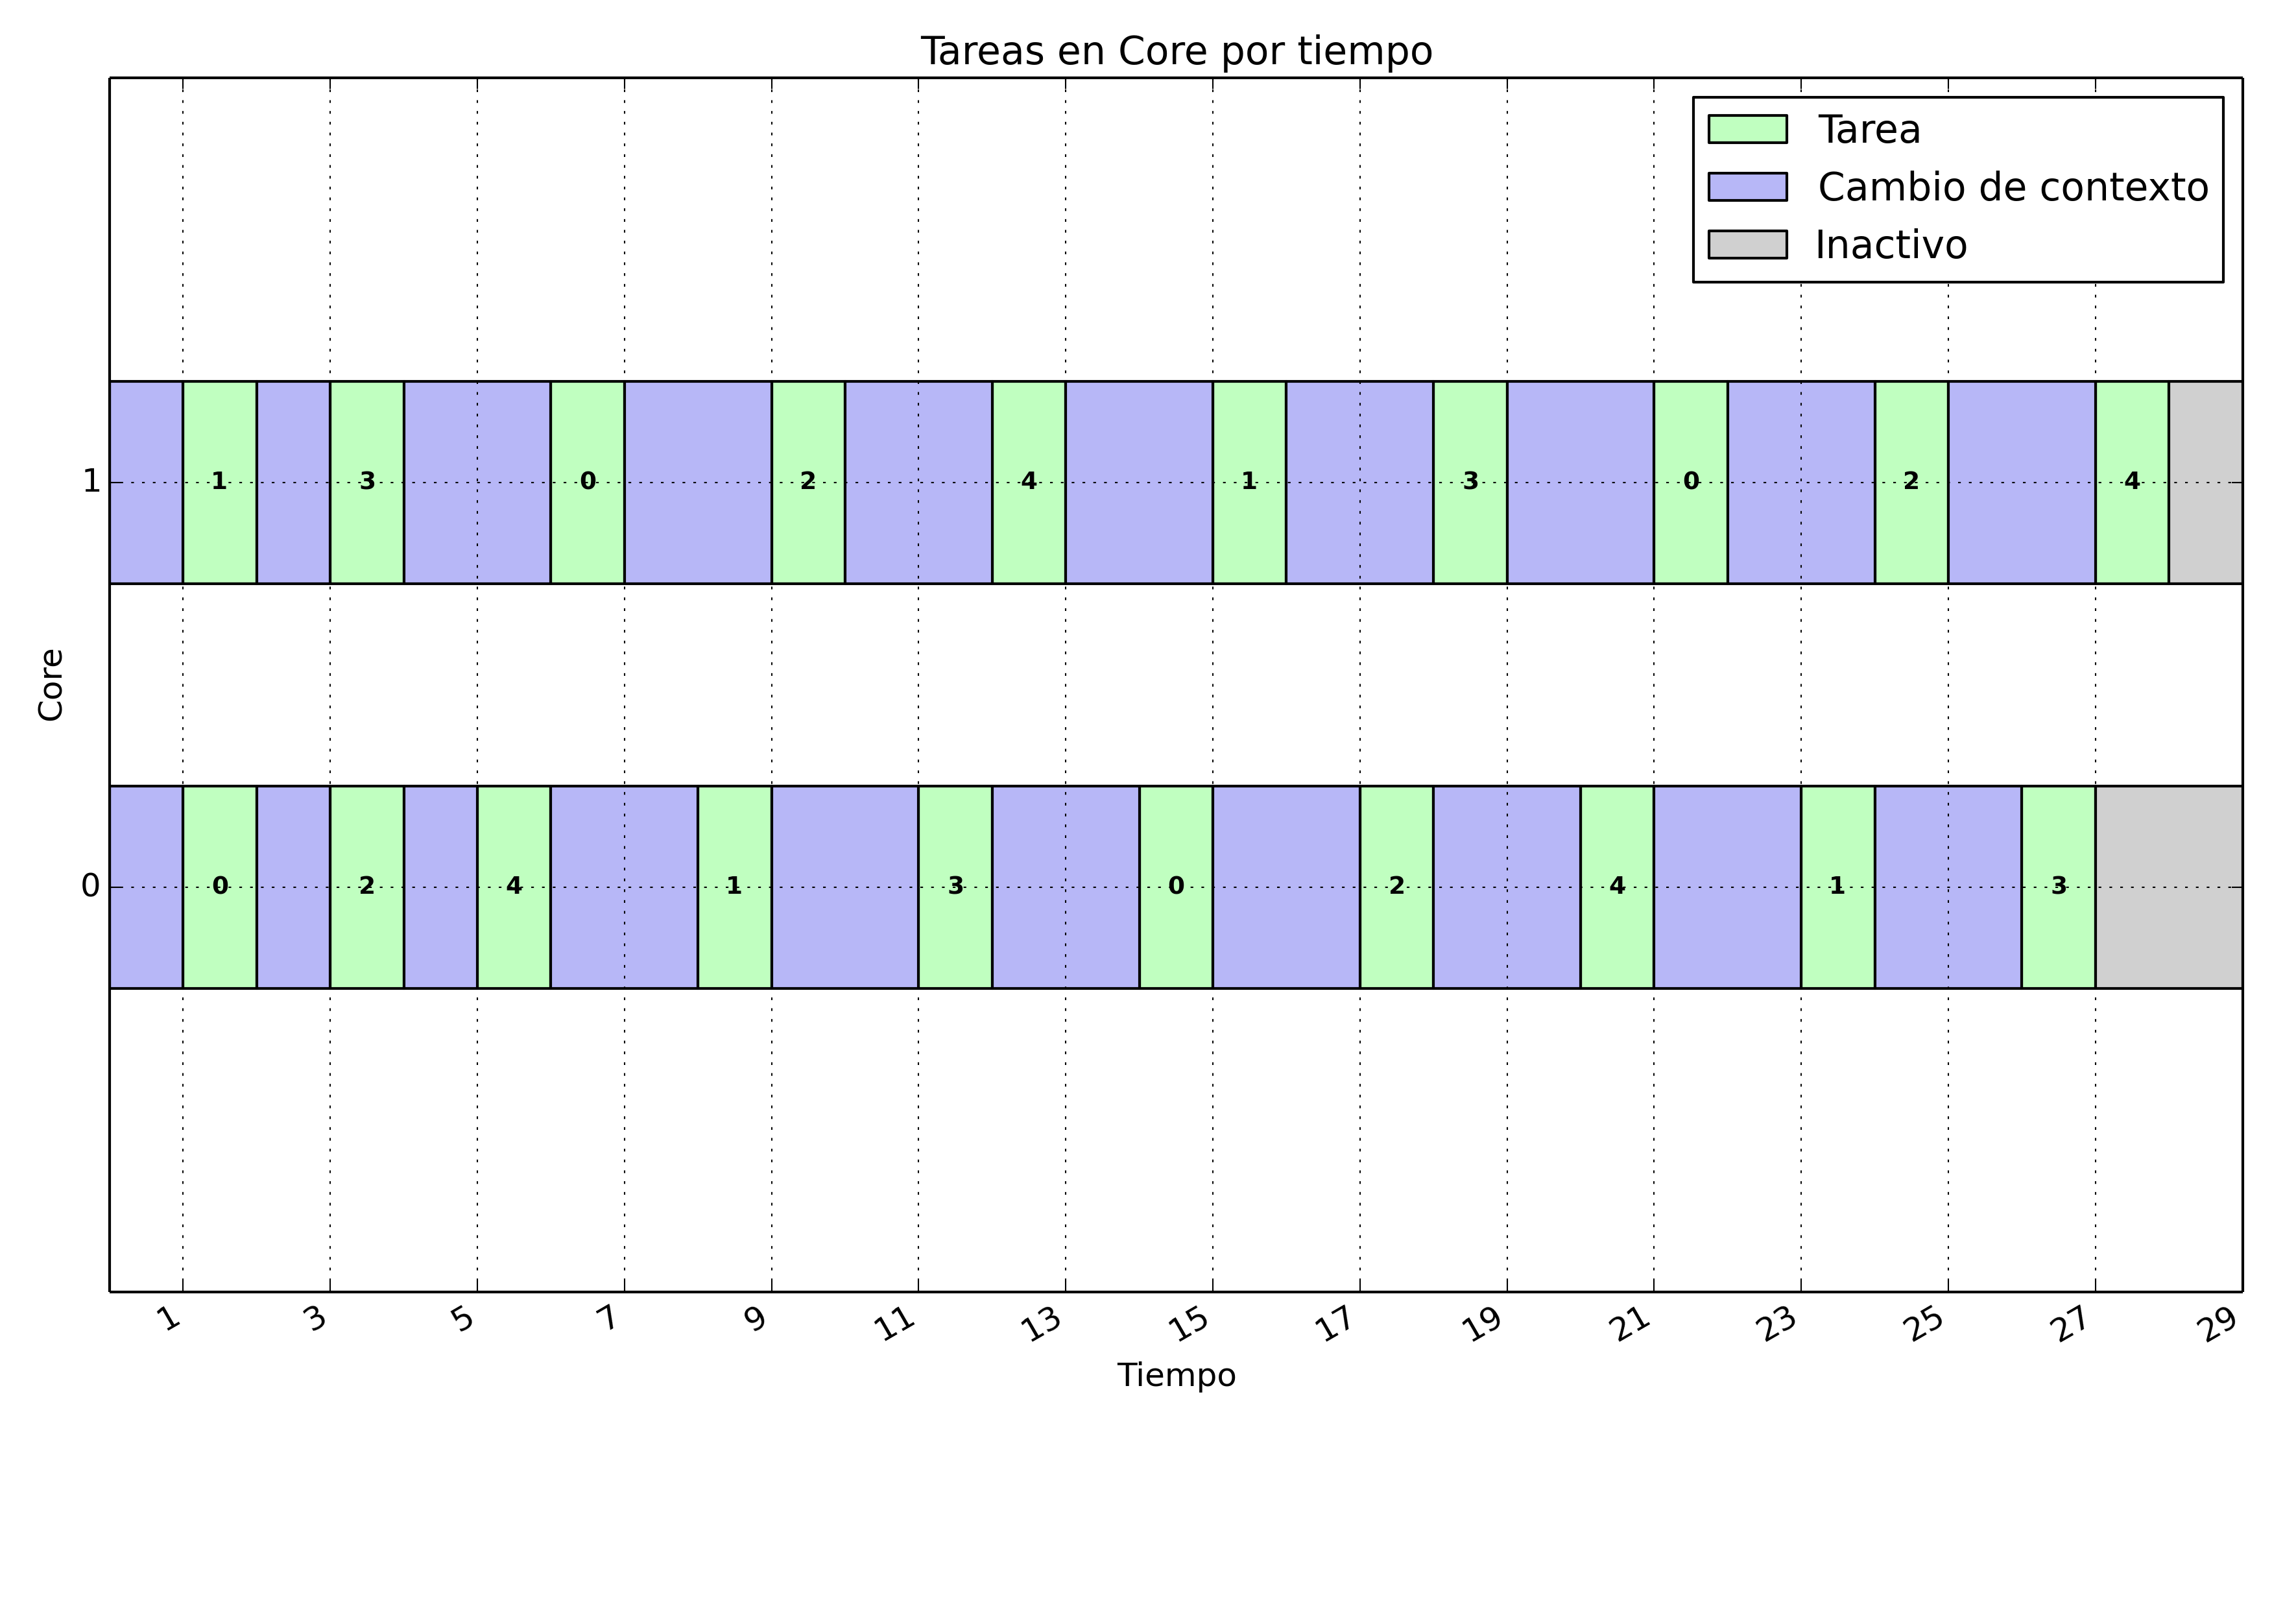
\includegraphics[width=\textwidth]{ejercicio_8_1}
\end{figure}

\begin{figure}[H]
\caption{SchedRR2 5 TaskCPU 2 cores 1 para cambio de core}
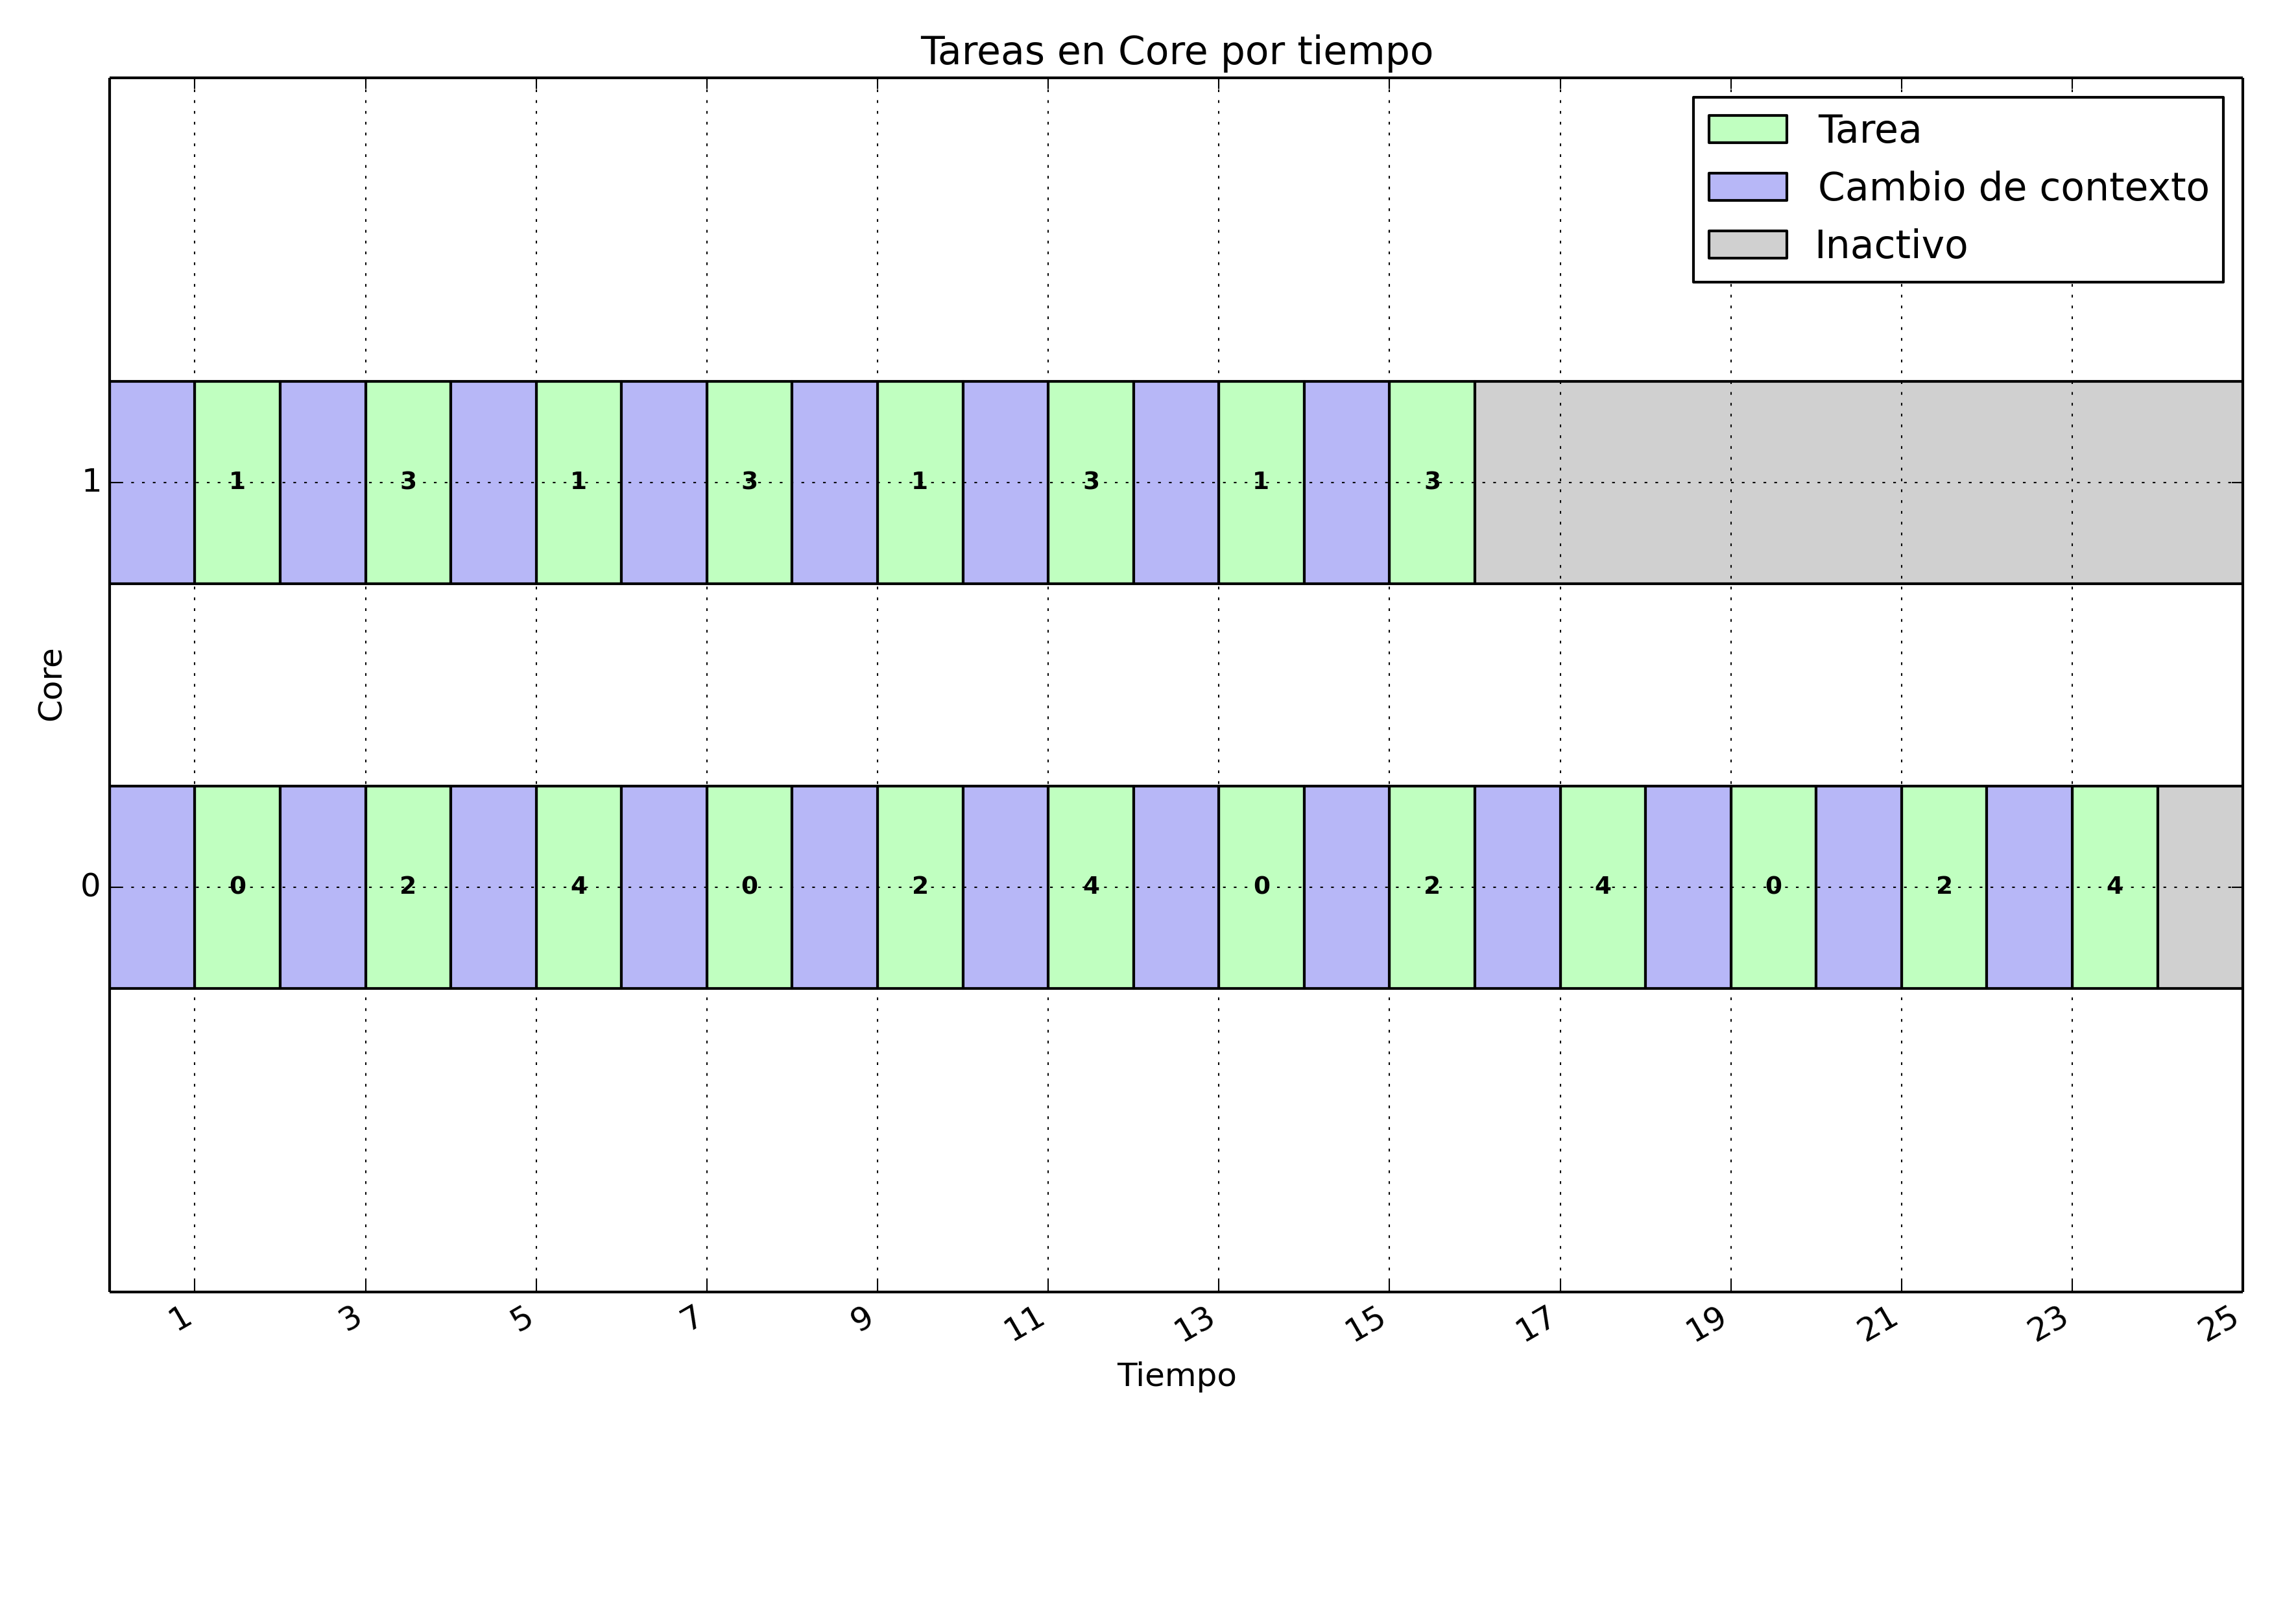
\includegraphics[width=\textwidth]{ejercicio_8_2}
\end{figure}


\begin{figure}[H]
\caption{SchedRR2 5 TaskCPU 2 cores 2 para cambio de core}
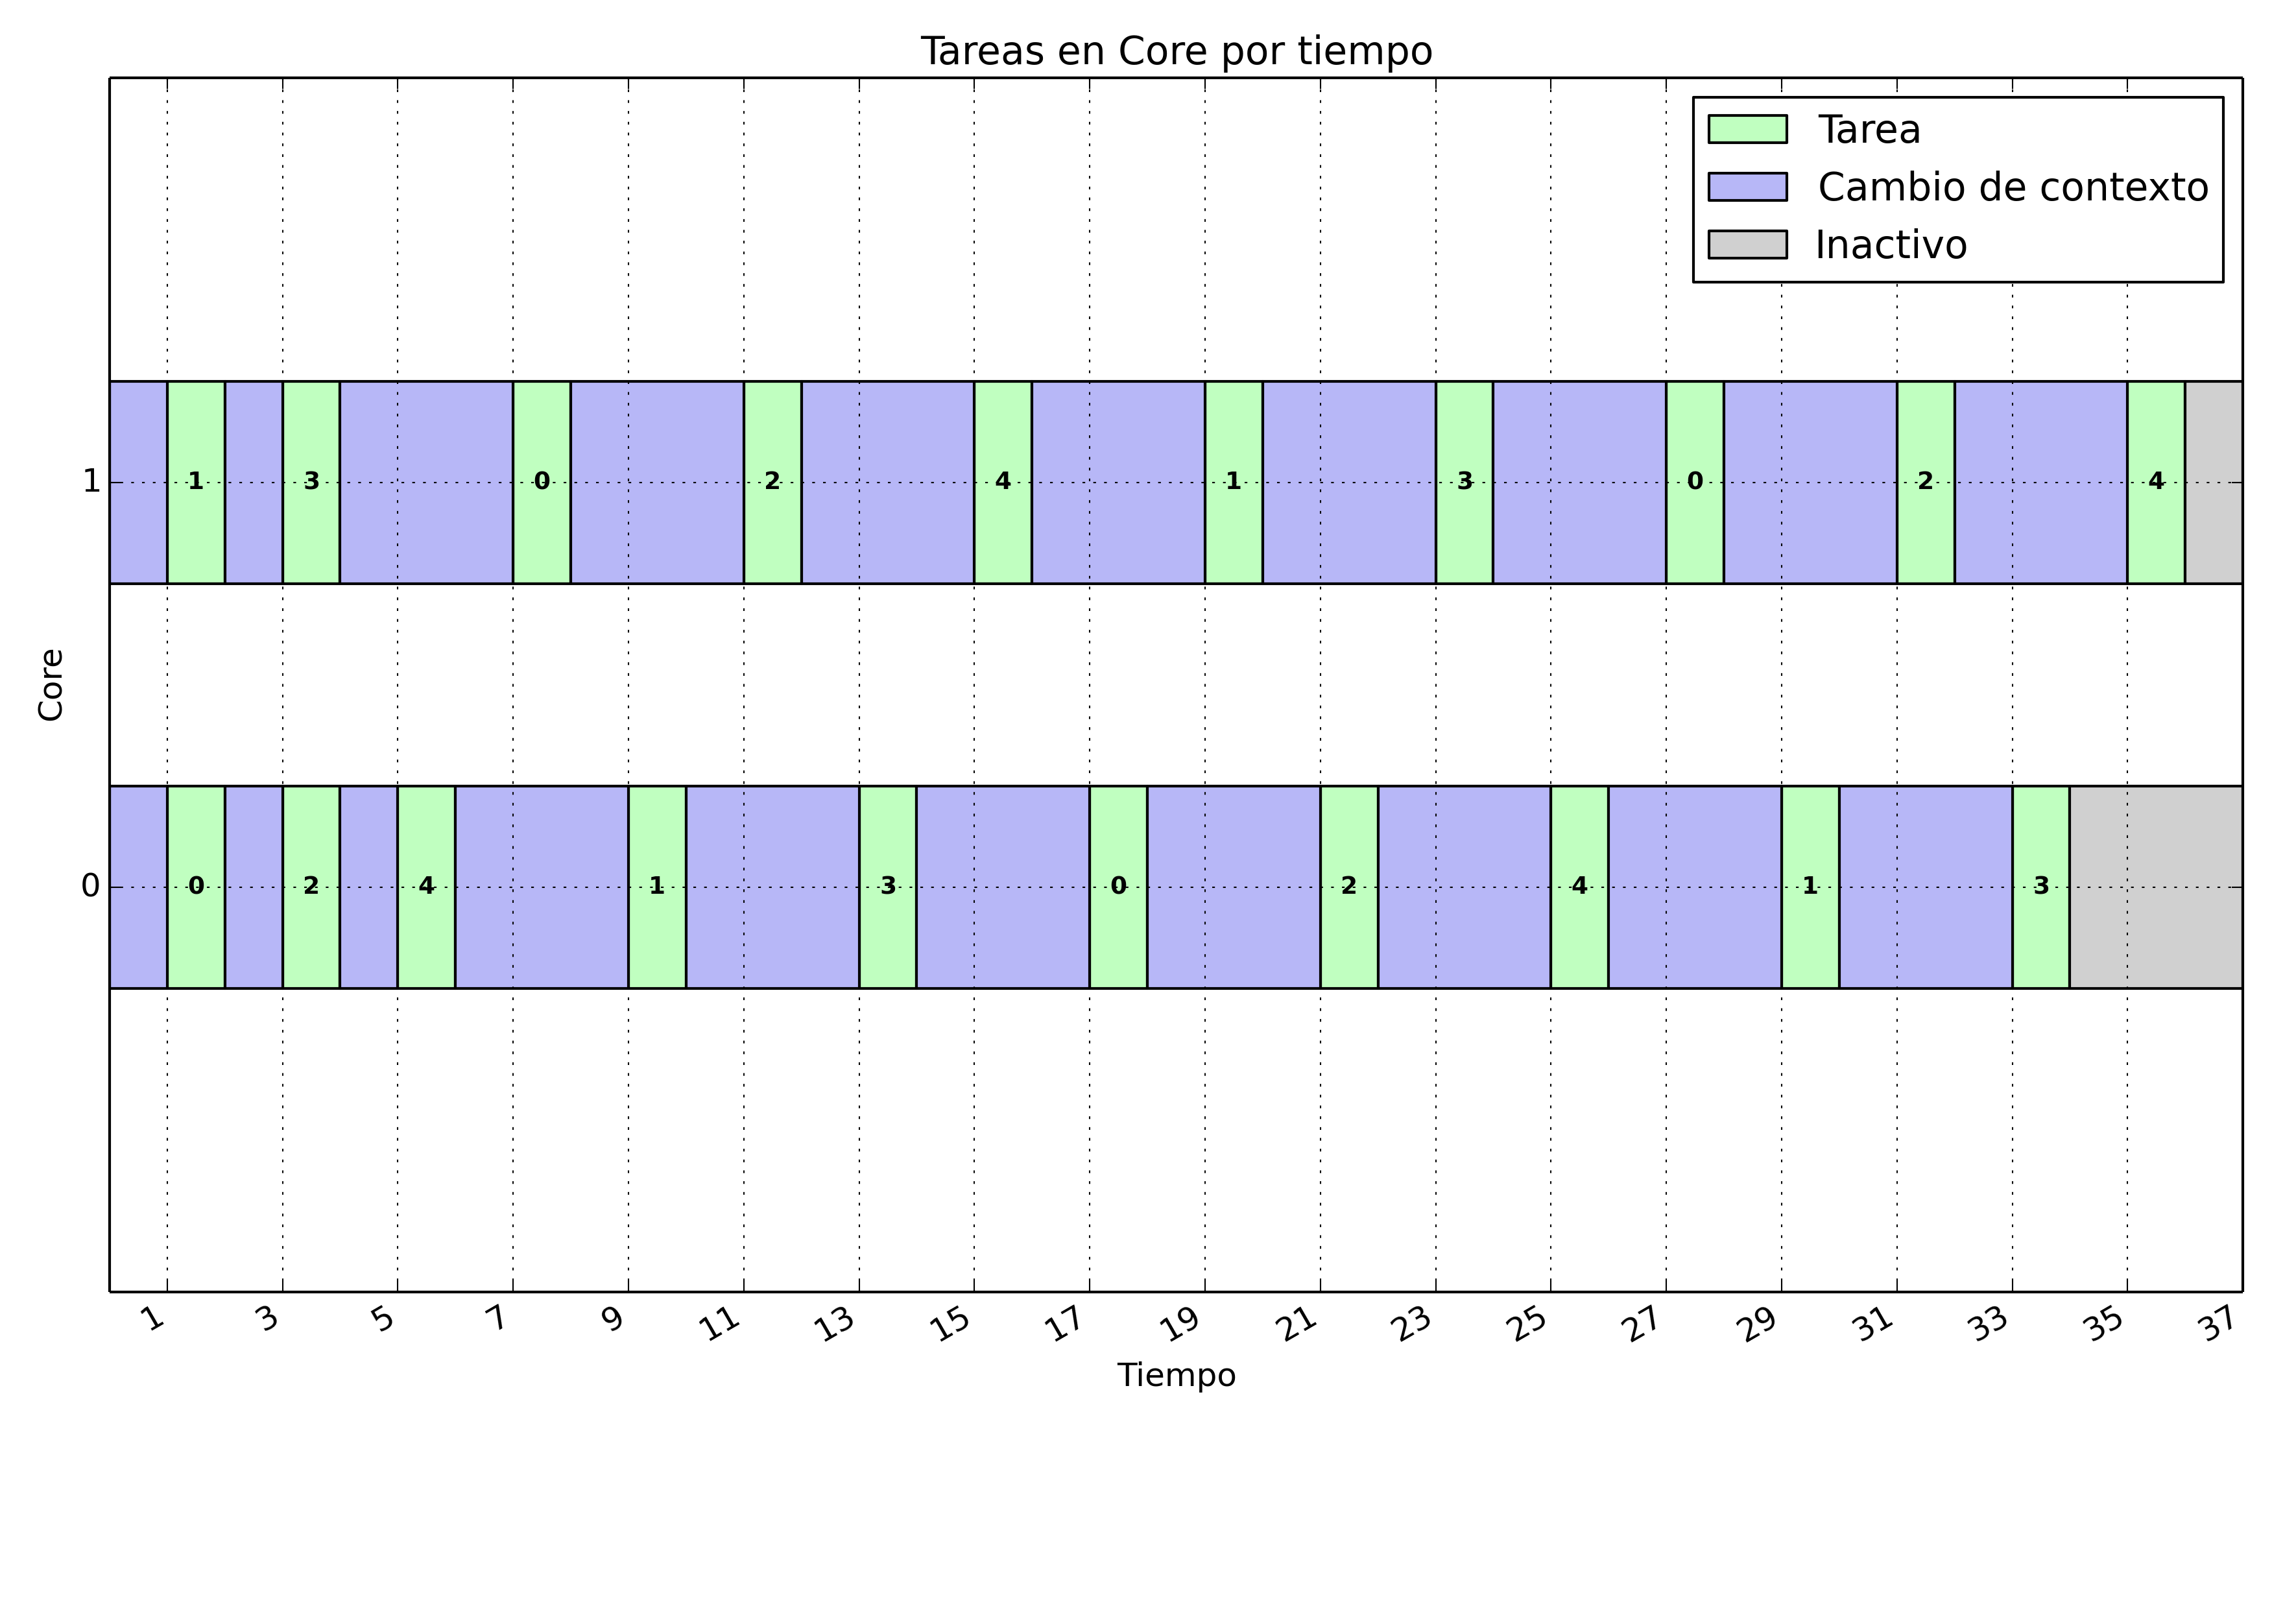
\includegraphics[width=\textwidth]{ejercicio_8_3}
\end{figure}


\begin{figure}[H]
\caption{SchedRR2 5 TaskCPU 2 cores 3  para cambio de core}
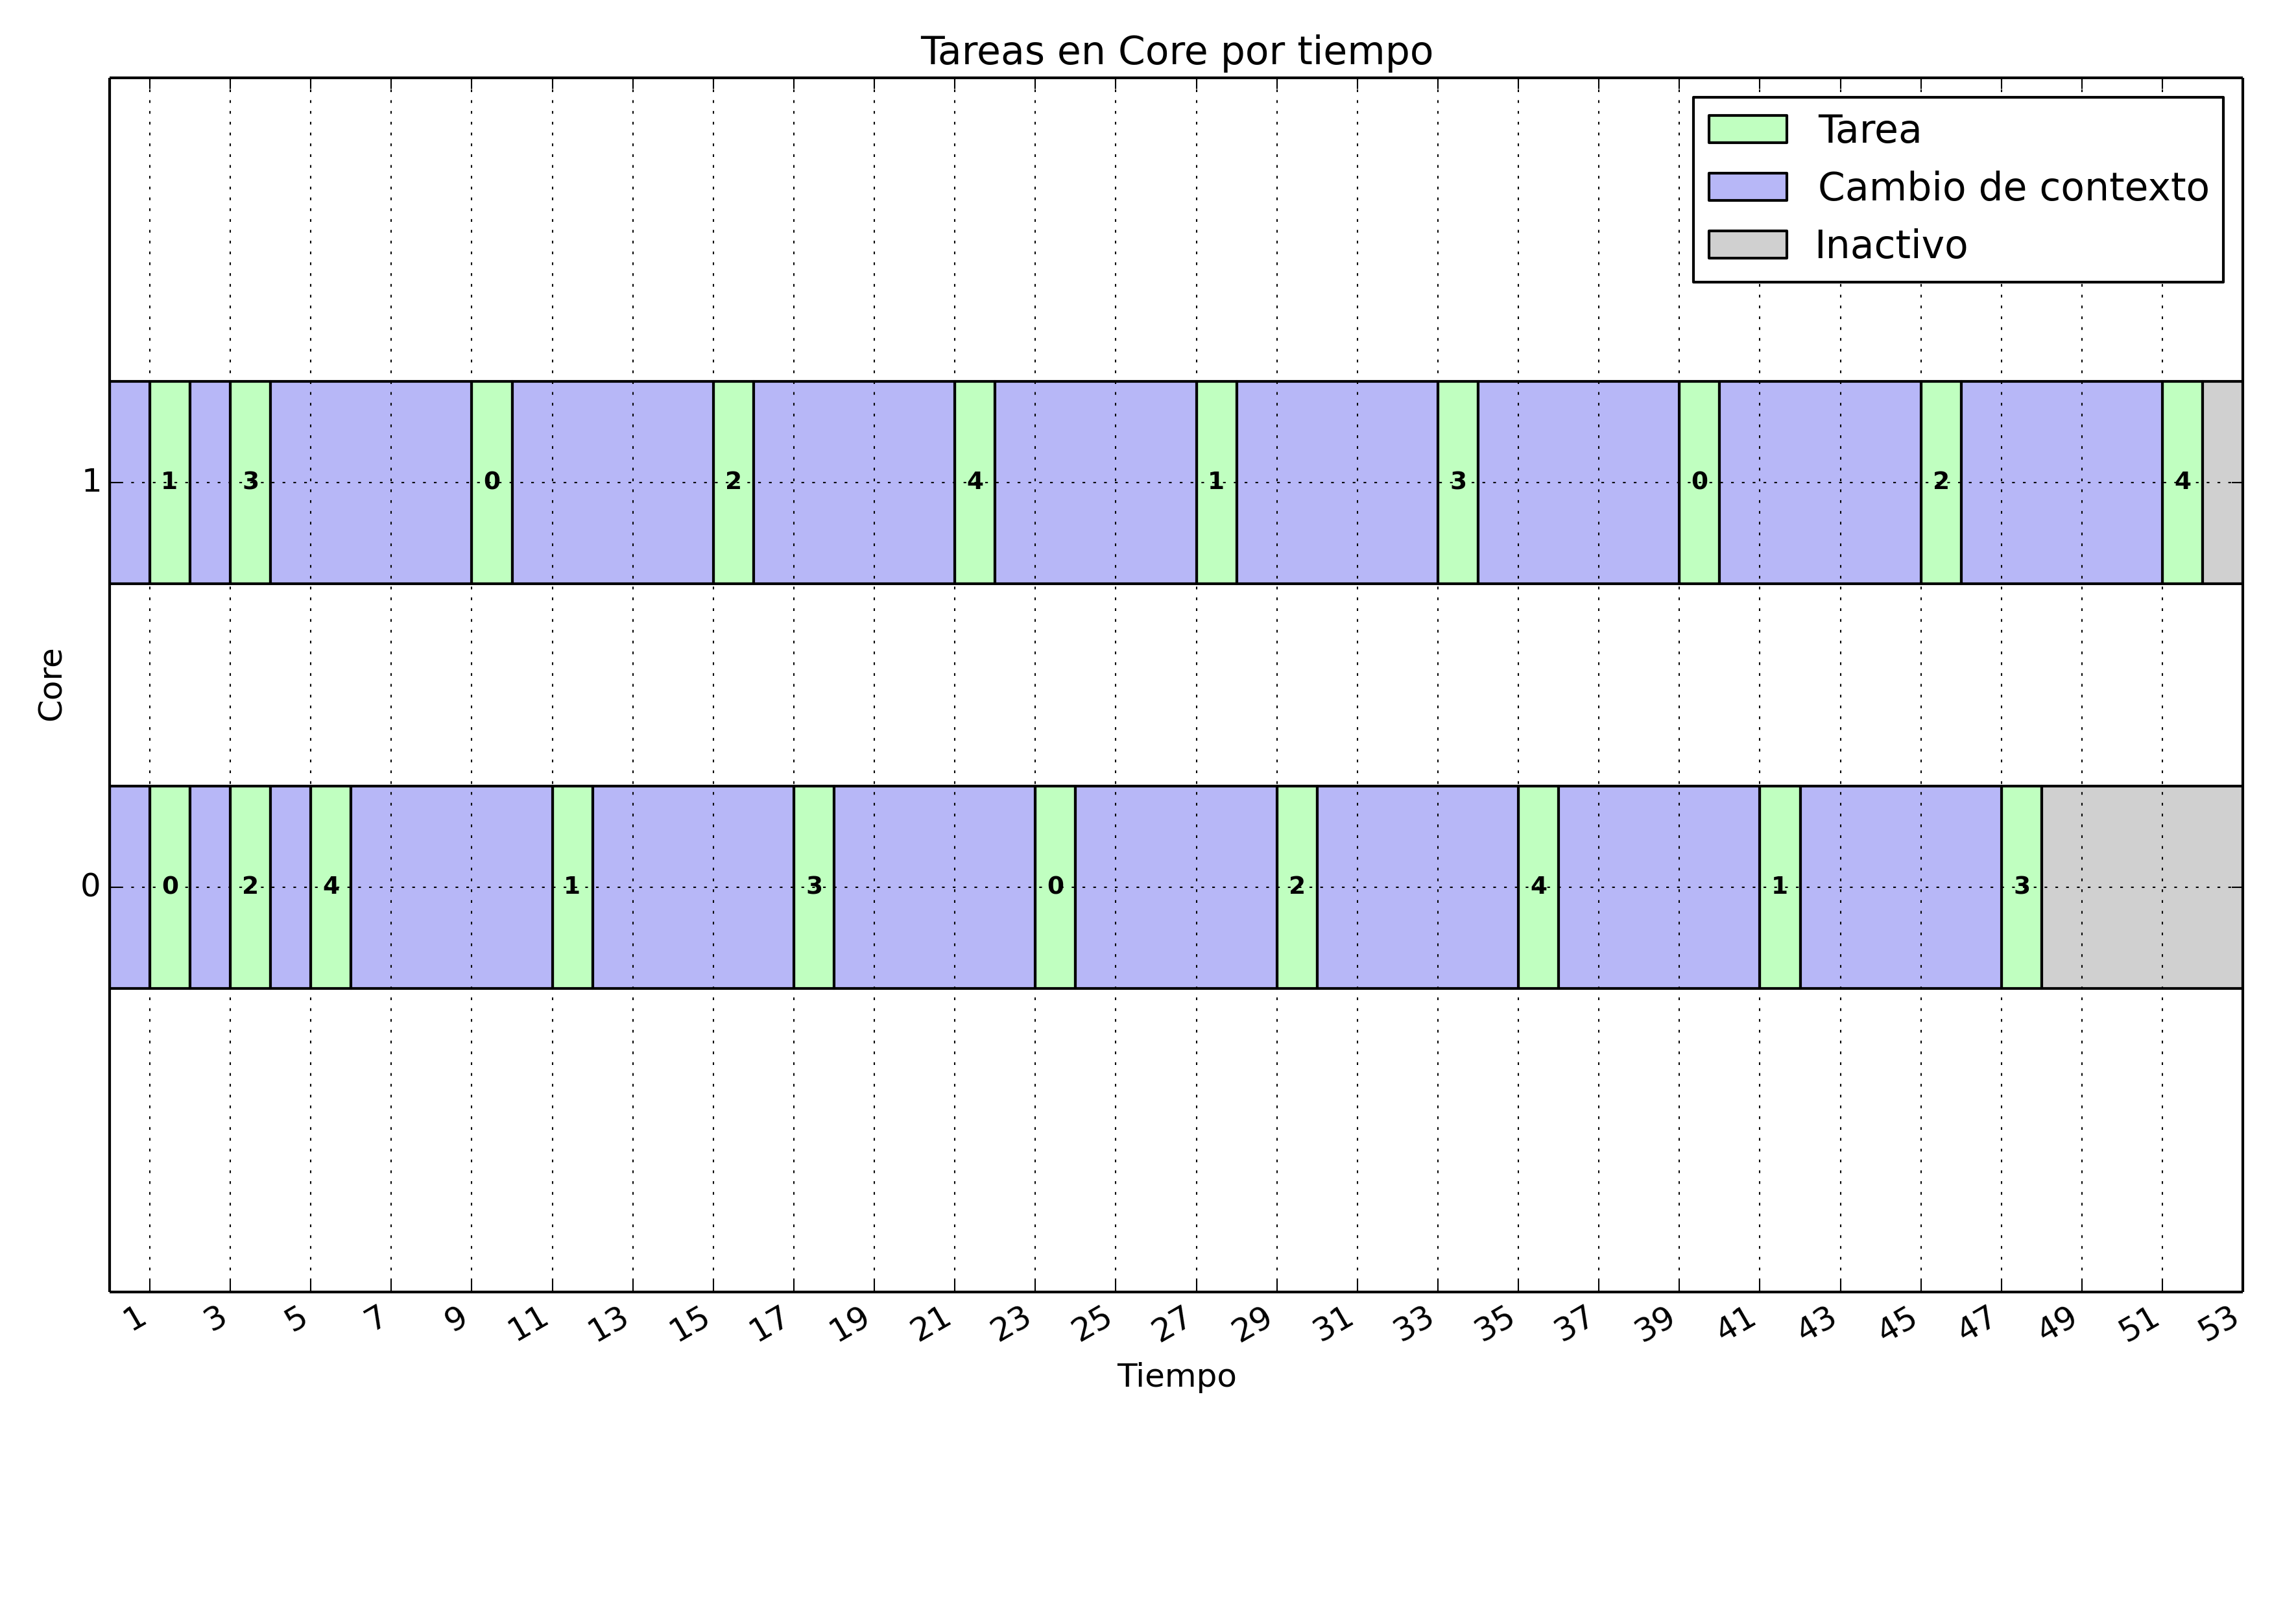
\includegraphics[width=\textwidth]{ejercicio_8_4}
\end{figure}

Se observa que el tiempo de turnaround promedio va aumentando en la medida en que aumenta el costo del cambio de core para SchedRR, mientras que en SchedRR2 se mantiene estable, ya que cada una de las tareas se mantiene asociada a una cola.
